%%%%%%%%%%%%%%%%%%%%%%%%%%%%%%%%%%%%%%%%%%%%%%%%%%%%%%%%%%%%%%%%
%% SECTION Analysis of Optimal Designs --- Vanishing Model Error
%%%%%%%%%%%%%%%%%%%%%%%%%%%%%%%%%%%%%%%%%%%%%%%%%%%%%%%%%%%%%%%%
\section{Analysis of D-Optimal Designs --- Vanishing Model Error}\label{section:vanishing}
\subsection{Overview}
In this section we analyze D-optimal designs when no model error is
present. Sensor clusterization is discussed in section
\ref{section:clusterization}. We first derive a nonlinear eigenvalue
problem in $\obs$ for D-optimal designs in Section
\ref{subsec:eigenproblem}. In Section \ref{subsec:characterization} we
characterize D-optimal designs as ones that make all eigenvalues equal
in the nonlinear eigenvalue problem. Results are summarized in Theorem
\ref{thm:char}.


\subsection{The Nonlinear Eigenvalue Problem}\label{subsec:eigenproblem}
$\modcov = 0$ implies $\Sigma= \sigma^2I$. The necessary first-order
condition for D-optimality \eqref{eq:conditions} becomes
\begin{equation}\label{eq:eigenproblem}
  \sigma^{-2}\fwd \postcov \fwd^* \obs^* = \obs^* \Xi,
\end{equation}
with $\Xi$ diagonal. We think of \eqref{eq:eigenproblem} as an
eigenvalue problem for the self-adjoint operator $\sigma^{-2}\fwd
\postcov \fwd^*$, where rows of $\obs$, namely $\meas_j,j=1,\dots, m$,
are eigenvectors. However, that $\postcov$ depends on $\obs$ and thus,
we refer to \eqref{eq:eigenproblem} as a nonlinear eigenvalue problem.

The following two lemmas allow us to gain better understanding of the
nonlinear eigenvalue problem.

\begin{restatable*}[Two applications of Woodbury Matrix Identity]{lemma}{woodbury}\label{lemma:twice woodbury}
  Assume $\fwd \prcov \fwd^*$ is invertible. Then
  \begin{align*}
    \begin{split}
      \fwd( \prcov^{-1} + \sigma^{-2}  \fwd^* \obs^* \obs \fwd )^{-1} \fwd^* 
      %
      %
      = \left ( (\fwd\prcov\fwd^*)^{-1} + \sigma^{-2}  \obs^* \obs \right )^{-1},
    \end{split}
  \end{align*}  
\end{restatable*}


%% The term $(\fwd \prcov \fwd^*)^{-1}$ is the prior precision in
%% $\hilo$, and $\fwd\prcov\fwd^*$ is invertible, as mentioned in
%% Section \ref{section:prelim}. $(\fwd\prcov\fwd^*)^{-1} + \sigma^{-2}
%% \obs^* \obs$ is the posterior precision in $\hilo$.

%% \subsection{Characterizing D-Optimal Designs}\label{subsec:characterization}
%% %% Denote corresponding eigenvectors $\{\ev_i\}_{i=1}^{\infty}$.
%% Denote eigenvalues of $\fwd \prcov \fwd^*$ by
%% $\{\lambda_i\}_{i=1}^{\infty}$, and note they are positive. Lemma
%% \ref{lemma:sim diag} is crucial for the rest of the analysis:

\begin{restatable*}[Simultaneous diagonizability for the nonlinear eigenvalue problem]{lemma}{simdiag}\label{lemma:sim diag}
  Let $\hil$ separable Hilbert space, $C:\hil \to \hil$ self-adjoint
  and $\func_1,\dots,\func_m \in \hil$. Denote $\func^*$ the element
  $\func$ acting as a linear functional. If
  \begin{equation*}
   (C + \sum_{j=1}^m \func_j\func_j^*) \func_l = \xi_l \func_l,\ l = 1,\dots,m
  \end{equation*}
  then $C$ and $\sum_{j=1}^m \func_j \func_j^*$ are simultaneously
  diagonalizable.
\end{restatable*}

\begin{corollary}[Eigenvectors of a D-optimal design]\label{cor:same ev}
  Let $\obs$ satisfy the nonlinear eigenvalue problem
  \eqref{eq:eigenproblem}. Then $\obs^*\obs$ has the same eigenvectors
  as $\fwd \prcov \fwd^*$.
\end{corollary}
\begin{proof}
  \begin{align}\label{eq:mod conditions}
    \begin{split}
      \obs^* \Xi &= \sigma^{-2}\fwd \postcov \fwd^* \obs^*  \text{ (by \eqref{eq:eigenproblem})}\\
      %
      %
      %
      &= \sigma^{-2} \fwd( \prcov^{-1} + \sigma^{-2}  \fwd^* \obs^* \obs \fwd )^{-1} \fwd^* \obs^*  \text{ (by \eqref{eq:postcov})} \\
      %
      %
      %
      &= \sigma^{-2} \left ( (\fwd\prcov\fwd^*)^{-1} + \sigma^{-2}  \obs^* \obs \right )^{-1} \obs^* \text{ (by Lemma \ref{lemma:twice woodbury})}.
    \end{split}
  \end{align}

  Now take $\func_j^{*} = \meas_j$ and $C := (\fwd \prcov
  \fwd^*)^{-1}$ and use Lemma \ref{lemma:sim diag}.
\end{proof}

%% Corollary \ref{cor:same ev} is important because it allows us to only think

implies we only need to consider $\obs$ such that  
At most $m$ of the eigenvectors of $\obs^*\obs$ have a positive
eigenvalue, because $k := \rank \obs^*\obs \leq m$. Since we made no
assumption regarding the ordering of $\{\lambda_i\}$, we can denote
the corresponding non-zero eigenvalues of $\obs^*\obs$ by
$\{\eta_i\}_{i=1}^{k}$ and let $\eta_i = 0$ for $i \geq k+1$.

%% \begin{definition}
%%   Let $\{\lambda_i\}_{i=1}^{\infty}$ eigenvalues of $\fwd \prcov
%%   \fwd^*$ sorted in descending order. Let $\eta \in
%%   \mathbb{R}_+^m$. The \emph{utility proxy} $\bar{\tar}$ is defined
%%   as:
%%   \begin{equation*}
%%     \bar{\tar}(\eta) := \frac12 \sum_{i=1}^m \log(1 + \sigma^{-2}\lambda_i\eta_i).
%%   \end{equation*}
%% \end{definition}

\begin{corollary}\label{cor:true target}
  Let $\obs$ with $m$ observations satisfy the nonlinear eigenvalue
  problem \eqref{eq:eigenproblem}. Let $\{\eta_i\}_{i=1}^{\infty}$
  eigenvalues of $\obs^*\obs$ and $\{\lambda_i\}_{i=1}^{\infty}$ the
  corresponding eigenvalues of $\fwd \prcov \fwd^*$. Let $k:=\rank
  \obs^*\obs$. Without loss of generality, let $\eta_i > 0$ for $i\leq
  k$ and $\eta_i = 0$ for $i > k$. Then:
  \begin{enumerate}
    \item $k \leq m$ and $\obs^*\obs$ has exactly $k$ positive
      eigenvalues.
    \item
      \begin{equation*}
        \tar(\obs) = \frac12 \sum_{i=1}^{k} \log (1 + \sigma^{-2}\lambda_i\eta_i) = \frac12 \sum_{i=1}^{m} \log (1 + \sigma^{-2}\lambda_i\eta_i).
      \end{equation*}
    \item Let $\obs$ a D-optimal design. Then $\eta_i > 0$ for
      eigenvectors corresponding to the $k$ largest $\lambda_i$.
  \end{enumerate}
\end{corollary}
\begin{proof}
  Part (1) is trivial. To see part (2) holds: 
  \begin{align}
    \begin{split}
      \tar(\obs) &= \frac12\log \det \left (I + \sigma^{-2} \prcov^{1/2} \fwd ^* \obs^*
      \obs \fwd \prcov^{1/2}\right )\\% \text{ (by definition)}\\
      %
      &= \frac12 \log \det \left (I + \sigma^{-2} \obs^* \obs \fwd
      \prcov\fwd^* \right ) \text{ (Sylvester's Determinant
      Theorem)}\\
      %
      %
      %
      &=\frac12 \log \prod_{i=1}^{\infty} ( 1 + \sigma^{-2} \lambda_i\eta_i ) \text{ (Corollary \ref{cor:same ev})} \\
      %
      %
      %
      %&=\frac12 \log \left ( \prod_{i=1}^{k} ( \lambda_i^{-1} + \sigma^{-2} \eta_i )\prod_{i=1}^{k} \lambda_i \right )
      %
      %
      %
      &=\frac12 \sum_{i=1}^{k} \log (1 + \sigma^{-2}\lambda_i\eta_i). 
      %
      %
      %% &=\frac12 \sum_{i=1}^{k} \log(\sigma^2\lambda_i^{-1} + \eta_i) - k\log \sigma + \frac12\sum_{i=1}^k \log \lambda_i.
    \end{split}
  \end{align}
  Part (3) holds since $\log$ is increasing and $\eta_i \geq 0$.
\end{proof}


\begin{proposition}\label{prop:kkt}
  Let $\tar: \mathbb{R}^m \to \mathbb{R}$, $\psi(\eta) =
  \frac{1}{2}\sum_{i=1}^m \log (1+\sigma^{-2}\lambda_i \eta_i)$, with
  $\lambda_i > 0$ and $\sigma^{2} > 0$. Then the maximum of $\tar$
  subject to $\eta_i \geq 0$ and $\sum\eta_i = m$ is obtained at
  \begin{equation}
  \eta_i = \begin{cases}
    \frac{m}{k} - \sigma^2 \lambda_i^{-1} + \sigma^2 \frac{1}{k} \sum_{j\in A} \lambda_j^{-1} & i \in A \\
    0 & i \in A^c
  \end{cases}
  \end{equation}
  where $A:= \{1\leq i \leq m: \eta_i > 0\}$ and $A^c = \{1,\dots, m\}
    \backslash A$, and $|A|$ is the cardinality of $A$.
\end{proposition}
\begin{proof}
%% \begin{proposition}\label{prop:optimizer}
%%   Let $\{\lambda_i\}_{i=1}^{\infty}$ the sorted eigenvectors of $\fwd
%%   \prcov\fwd^*$, $k\in \mathbb{N}^+$ and
%%   %% Let
%%   %%   \begin{equation}
%%   %%   k = \argmax \left \{ k:\lambda_k^{-1} \leq \sigma^{-2}\frac{m}{k} + \frac{1}{k} \sum_{j=1}^{k}
%%   %%   \lambda_j^{-1} \right \}.
%%   %% \end{equation}

%%   \begin{equation}
%%   \eta_i = \begin{cases}
%%     \frac{m}{k} - \sigma^2 \lambda_i^{-1} + \sigma^2 \frac{1}{k} \sum_{j=1}^k \lambda_j^{-1} & i \leq k \\
%%     0 & i > k 
%%   \end{cases}.
%%   \end{equation}

%%   Let $\obs$ an observation operator such that $\obs^*\obs$ has the
%%   same eigenvectors as $\fwd \prcov \fwd^*$. If $\eta_i > 0$ for
%%   $i\leq k$ and $\obs^*\obs$ has eigenvalues $\eta_i$, then $\obs$
%%   maximizes $\tar$ subject to $\sum_{i=1}^m \eta_i = m$ and to $\rank
%%   \obs = k$.
%% \end{proposition}
  %% \begin{proof}
  %% et $A := \{i: \eta_i > 0\}$. A choice of $A$ where $\eta_i =0,
  %% \eta_j >0$ for some $1 \leq i < j \leq m$ is not optimal (just
  %% switch $\eta_j$ and $\eta_i$ and recall $\{\lambda_i\}$ are arranged
  %% in descending order). Thus, since $\rank \obs = k$ we conclude that,
  %% $\eta_i=0, i>k$.

  Let $\Phi(\eta) = \sum_{i=1}^k \eta_i - m$ and $\Omega_j(\eta) =
   -\eta_j$. Then
  \begin{align*}
    \begin{split}
      \frac{\partial \tar}{\partial \eta_i}  &=
       \frac12 \frac{\sigma^{-2}\lambda_i}{1 + \sigma^{-2} \lambda_i\eta_i} = \frac12 \frac{1}{\sigma^{2}\lambda_i^{-1} + \eta_i} \\
      %
      %
      %
      \frac{\partial\Phi}{\partial \eta_i} &= 1 \\
      %
      %
      %
      \frac{\partial \Omega_j}{\partial \eta_i} &= -\delta_{ij}      
    \end{split}
  \end{align*}

  From the KKT conditions, there are $\alpha, \beta_i$ such that for $i=1,\dots,m$:
  \begin{align}
    \begin{split}
      -\frac12 \frac{1}{\sigma^{2}\lambda_i^{-1} + \eta_i} + \alpha - \beta_i  &= 0 \\
      %
      %
      %
      \eta_i &\geq 0\\
      %
      %
      %
      \beta_i &\geq 0\\
      %
      %
      %
      \beta_i \eta_i &= 0\\
      %
      %
      %
      \sum_{i=1}^m \eta_i &= m 
    \end{split}
  \end{align}

  Then, for $i \in A$:
  \begin{align*}
    \begin{split}
      \beta_i &= 0\\
      %
      %
      %
      \sigma^{2}\lambda_i^{-1} + \eta_i  &= \frac{1}{2\alpha}%  \text{ for }  1 \leq i \leq k.\\
      %
      %
      %
      %% \sigma^{-2} \lambda_i &= 2\alpha - 2\beta_i, i \in B \\
    \end{split}
  \end{align*}
  
  Summing over $i \in A$, substituting $\sum_{i\in A} \eta_i =
  \sum_{i=1}^m \eta_i = m$, and dividng by $k:= |A|$:
  $$
  \frac{1}{2\alpha} = \frac{m}{k} + \frac{\sigma^2}{k} \sum_{j\in A} \lambda_j^{-1}.
  %\Rightarrow \alpha = \left ( \frac{2m}{k} + \frac{2\sigma^2}{k}
  %\sum_{i\in A} \lambda_i^{-1} \right )^{-1}.
  $$

  Consequently:
  \begin{align} \label{eq:etas}
    \begin{split}
      \eta_i &= \frac{1}{2\alpha} - \sigma^2 \lambda_i^{-1}\\
      %
      %
      %
      &=\frac{m}{k} + \frac{\sigma^2}{k} \sum_{j\in A} \lambda_j^{-1} - \sigma^2 \lambda_i^{-1}.%\\
      %
      %
      %
      %% &= \frac{m}{k} + \frac{\sigma^2}{k} \sum_{j \in A, j\neq i} \lambda_j^{-1} - \frac{k-1}{k}\sigma^2 \lambda_i^{-1}\\
      %% ,\ i \in A.
    \end{split}
  \end{align}
\end{proof}

\begin{corollary}\label{cor:descending}
  In Proposition \ref{prop:kkt}, if $\lambda_i$ are arranged in
  descending order, then $A= \{1,\dots,k\}$ for some $1 \leq k \leq
  m$.
\end{corollary}

\begin{corollary}\label{cor:eigenvalues}
  If $\obs$ is optimal and $k := \rank \obs$, then:
  \begin{enumerate}
    \item The covariance of the pushforwad $\fwd_{*} \post$ is $((\fwd
      \prcov \fwd^*)^{-1} + \sigma^{-2} \obs^*\obs)^{-1}$.
    \item The eigenvalues of said operator are
      \begin{equation}
        \eta_i = \begin{cases}
          \frac{m}{k} + \sigma^2 \frac{1}{k} \sum_{j=1}^k \lambda_j^{-1} & i \leq k \\
          \lambda_i^{-1} & i > k 
        \end{cases}.
      \end{equation}
  \end{enumerate}
\end{corollary}

\begin{proof}
  Recall from \eqref{eq:postcov}, that the posterior covariance is
  $\postcov^{-1} = \prcov^{-1} +
  \sigma^{-2}\fwd^*\obs^*\obs\fwd$. Part (1) now follows from Lemma
  \ref{lemma:twice woodbury}. Part (2) follows from Propositin
  \ref{prop:kkt} and Corollary \ref{cor:descending}.
\end{proof}

We are almost ready to state and prove Theorem \ref{thm:char} that
characterizes D-optimal designs. We just need one final lemma, whose
proof is delegated to the appendix:
\begin{restatable*}[Unit norm decomposition]{lemma}{free}\label{lemma:free}
  Let $M \in \R^{k \times k}$ symmetric positive definite with $\ttr M
  = m$, $m \geq k$. We can find $\func_j \in \R^k,j=1,\dots,m$
  with $\|\func_j\|=1$ and $A = (\func_1,\dots,\func_m)$ such that
  $AA^t = M$.
\end{restatable*}


\main

\begin{proof}
  Part (1) was proved in Corollary \ref{cor:same ev}. Parts (2) and
  (3) were proved in Corollary \ref{cor:true target}. Part (4) is a
  consequence Corollariy \ref{cor:eigenvalues}, with the caveat that
  we did not show that finding $\obs$ so that $\obs^*\obs$ has the
  desired eigenvalues is feasible. To this end, we utilize Lemma
  \ref{lemma:free}: let $M = \diag(\eta_1, \dots, \eta_k)$, diagonal
  with respect to the first $k$ eigenvectors of $\fwd \prcov
  \fwd^*$. We take $\obs := A$ from the Lemma \ref{lemma:free}, and
  this concludes the proof.
\end{proof}

\begin{corollary}
  In a D-optimal design, the posterior precision for eigenvector $i$
  is $\eta_i + \sigma^2 \lambda_i^{-1} = \frac{m}{k} + \sigma^2
  \frac{1}{k} \sum_{j=1}^k \lambda_j^{-1}$. I.e. the posterior
  precision in $\hil_p$ is constant for $1 \leq i \leq k$, where $k
  =\rank \obs$.
\end{corollary}

\pgfplotstableread{
  Label     prior  optimal  sub-optimal 
  1         0.2    1.8           1.7
  2         0.8    1.2           0.8
  3         2.2    0             0.5
  4         3.5    0             0.0
}\optimalvsnot

\begin{figure}
  \begin{tikzpicture}[scale=0.85]
    \begin{axis}[
        ybar stacked,
        ymin=0,
        ymax=4,
        xtick=data,
        legend style={cells={anchor=east}, legend pos=north west, legend columns=-1},
        reverse legend=false, % set to false to get correct display, but I'd like to have this true
        xticklabels from table={\optimalvsnot}{Label},
        xticklabel style={text width=2cm,align=center},
        legend plot pos=right,
        ylabel=precision --- prior and posterior,
        xlabel=eigenvector $i$,
      ]
    
      
      \addplot [fill=green!80]  table [y=prior,   meta=Label, x expr=\coordindex] {\optimalvsnot};
      \addplot [fill=blue!60]   table [y=optimal, meta=Label, x expr=\coordindex] {\optimalvsnot};
            
      \addlegendentry{$\sigma^2\lambda_i^{-1}$}
      \addlegendentry{optimal $\eta_i$s}
      
    \end{axis}
  \end{tikzpicture}
  \qquad
  \begin{tikzpicture}[scale=0.85]
    \begin{axis}[
        ybar stacked,
        ymin=0,
        ymax=4,
        xtick=data,
        legend style={cells={anchor=east}, legend pos=north west, legend columns=-1},
        reverse legend=false, % set to false to get correct display, but I'd like to have this true
        xticklabels from table={\optimalvsnot}{Label},
        xticklabel style={text width=2cm,align=center},
        legend plot pos=right,
        ylabel=precision --- prior and posterior,
        xlabel=eigenvector $i$,
      ]   
      
      \addplot [fill=green!80]  table [y=prior,       meta=Label, x expr=\coordindex] {\optimalvsnot};
      \addplot [fill=blue!60]   table [y=sub-optimal, meta=Label, x expr=\coordindex] {\optimalvsnot};

      \addlegendentry{$\sigma^2\lambda_i^{-1}$}
      \addlegendentry{sub-optimal $\eta_i$s}
      
    \end{axis}
  \end{tikzpicture}
  \caption{As an illustration of Corollary \ref{cor:equal eigs}, a
    D-optimal design is compared with a sub-optimal design. Both
    designs are allowed three observations. Thus, the blue area has
    accumulated height of $3$ in both plots. A D-optimal design (left)
    increases precision (reduces uncertainty) where it is lowest. A
    sub-optimal design (right) does not. In this example, an
    observation is taken partly in the direction of the third
    eigenvector. The precision for this eigenvector is bigger even
    than the posterior precision of the D-optimal design on the left.}
  \label{fig:optimal vs not}
\end{figure}



\pgfplotstableread{
  Label    prior  $o_1$  $o_2$   $o_3$   $o_4$   $o_5$         $o_6$    topper
  1         0.2    0.8    0.5     0.5    0.4    0.33333333  0.3333333  0.001
  2         0.8    0.2    0.5     0.5    0.4    0.33333333  0.3333333  0.001
  3         2.2    0      0       0      0.2    0.33333333  0.3333333  0.001
  4         3.5    0      0       0      0      0           0          0.001
}\clusterization


\pgfplotstableread{
  Label    prior  $o_1$  $o_2$   $o_3$   $o_4$   $o_5$         $o_6$    topper
  1         0.2    0.8    0.7     0.3    0.4    0.2         0.4666666  0.001
  2         0.8    0.2    0.3     0.7    0.4    0.46666666  0.2        0.001
  3         2.2    0      0       0      0.2    0.33333333  0.3333333  0.001
  4         3.5    0      0       0      0      0           0          0.001
}\noclusterization

Here is a way to understand D-optimal designs with vanishing model
error: Imagine each eigenvector corresponds to a graduated lab
cylinder (Figure \ref{fig:cylinder}). Each cylinder $i$ is filled,
a-priori, with green liquid of $\sigma^2\lambda_i^{-1}$ volume
units. This liquid represnets the prior precision, weighted by
observation noise. The volume of the green liquid is increasing in
$i$. A D-optimal design with $m$ observations ignores cylinders
indexed $m+1$ and above. It has blue liquid of volume $m$ units at its
disposal. It distributes said liquid by repeatedly adding a drop to
whatever cylinder currently has the lowest level of liquid in it
(lowest precision). The result of such a procedure is illustrated in
Figure \ref{fig:optimal vs not}.

\begin{figure}%{r}{0.25\textwidth} 
    %\centering
    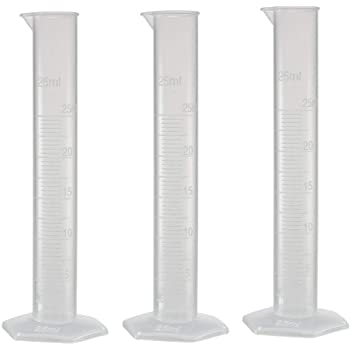
\includegraphics[width=5cm, height=5cm]{cylinders.jpg}
    \caption{Three graduated lab cylinders, corresponding to three
      eigenvectors. Prior eigenvalues not shown.}
    \label{fig:cylinder}
\end{figure}



\section{Sensor Clusterization --- Vanishing Model Error}\label{section:clusterization}
\subsection{Overview}
In this section we use Theorem \ref{thm:char} to explain how sensor
clusterization may arise in various scenarios. We first consider
sequential designs, and then simultaneous designs.


\subsection{Sequential Design}\label{subsec:clusterization sequential}
In a sequential optimal design problem, each measurement is taken
after results of previous measurements are recorded. In each step
$m=1$, so $k=1$. In this case, Theorem \ref{thm:char} implies each
measurement is taken along the direction of the eigenvector of $\fwd
\prcov \fwd^*$ with lowest posterior precision. If $\lambda_i$
decrease fast enough (e.g. exponentially), the

, $\meas_1 \parallel \ev_1$ and $\eta_1 = 1$. As hinted in
section \ref{subsec:seq vs sim}, the posterior becomes the prior for
the next step. The eigenvectors of the new posterior are the same as
for the previous one. A new observation will be taken in the direction
of eigenvector with smalles eigenvalue. This leads to:
\begin{align*}
  \begin{split}
    \meas_2 \parallel \ev_1  &\text{ if } \sigma^2 \lambda^{-1}_1 + 1 < \sigma^2\lambda^{-1}_2 \\
    \meas_2 \parallel \ev_2  &\text{ o.w. }
  \end{split}
\end{align*}
In the first case, we get clusterization immediately. In the second,
we consider $\meas_3$. Same reasoning leads to the conclusion that the
eigenvectors of the new prior precision are the same. The eigenvalues,
however, are $\lambda^{-1}_1 + \sigma^{-2}, \lambda^{-1}_2 +
\sigma^{-2}, \lambda_3^{-1}, \dots$. A new observation is taken in the
direction of eigenvector of smallest precision (note that
$\lambda^{-1}_1 + \sigma^{-2} < \lambda^{-1}_2 + \sigma^{-2}$):
\begin{align*}
  \begin{split}
    \meas_3 \parallel \ev_1 &\text{ if } \sigma^2 \lambda^{-1}_1 + 1 <
    \sigma^2\lambda^{-1}_3 \\
    \meas_3 \parallel  \ev_3  &\text{ o.w. }
  \end{split}
\end{align*}
Again, the first case results in clusterization. The sequential design
proceeds in this fashion. Every $\meas_i$ is taken in the direction
some eigenvector of the prior $\fwd \prcov\fwd^*$. This eigenvector
has the smallest eigenvalue of the previous step's posterior precision
operator. If we do not encounter clusterization after $m$ such steps,
this means that observation $\meas_k$ was taken in the direction
$\ev_k$ for $k=1,\dots,m$. Thus:
\begin{align}\label{eq:failure}
  \begin{split}
    \sigma^2\lambda_{k-1}^{-1} + 1 \geq \sigma^2\lambda_k^{-1}, \text{ for } 1\leq k \leq m
    \Longrightarrow \lambda_m^{-1} - \lambda_{m-1}^{-1} \leq \sigma^{-2}.
  \end{split}
\end{align}

But \eqref{eq:failure} implies $\{\lambda_i^{-1}\}_{i=1}^{\infty}$
grows at most linearly. In section \ref{subsec:abstract OED} we
assumed $\fwd$ is strongly smoothing, which means eigenvalues of
$(\fwd \prcov\fwd^*)^{-1}$ grow quickly. Thus, if we take $m$ large
enough, \eqref{eq:failure} will eventually fail and we will observe
sensor clusterization.


\subsection{Simultaneous Design}\label{subsec:clusterization simultaneous}
In a simultaneous design scenario, the result is not simple as in the
sequential design case. We now see that a design that exhibits
clusterization is as optimal as one that does not. Corollary
\ref{cor:same ev} tells us that we can realize any design we want
(encoded in $\{\eta_i\}$), given the trace constraint for
$\obs^*\obs$. Theorem \ref{thm:char} tells us that for D-optimality,
we only need to make the posterior flat where we take observations
(recall figure \ref{fig:optimal vs not}). We are left with the freedom
of assigning any part of $\eta_i$ to any observation $\meas_j$. Two
possible assignments for the same problem are illustrated in figure
\ref{fig:clusterization}. The first exhibits clusterization, the
second does not. It is important to note that neither arises as a
result of some numerical optimization scheme. Both designs give the
same design criterion $\tar$, because their posteriors are
identical. By Theorem \ref{thm:char}, both are maximizers of the same
D-optimal design problem. One exhibits clusterization, and one does
not. It is likely that a real-life problem is more restricted than the
model we consider here. Such restriction is the likely cause of
clusterization obseved in, e.g., the toy model of section
\ref{subsec:example}. Exactly how this happens is not clear. At this
point it is the subject of speculation and should be further studied
in the future.


\begin{figure}
  \begin{tikzpicture}[scale=0.85]
    \begin{axis}[
        ybar stacked,
        ymin=0,
        ymax=4,
        xtick=data,
        legend style={cells={anchor=east}, legend pos=north west, legend columns=-1},
        reverse legend=false, % set to false to get correct display, but I'd like to have this true
        xticklabels from table={\clusterization}{Label},
        xticklabel style={text width=2cm,align=center},
        legend plot pos=right,
        ylabel=precision --- prior and posterior,
        xlabel=eigenvector $i$,
      ]
    
      
      \addplot [fill=green!80]  table [y=prior, meta=Label, x expr=\coordindex] {\clusterization};
      \addplot [fill=blue!60]   table [y=$o_1$, meta=Label, x expr=\coordindex] {\clusterization};
      \addplot [fill=red!60]    table [y=$o_2$, meta=Label, x expr=\coordindex] {\clusterization};
      \addplot [fill=black!60]  table [y=$o_3$, meta=Label, x expr=\coordindex] {\clusterization};
      \addplot [fill=orange!60] table [y=$o_4$, meta=Label, x expr=\coordindex] {\clusterization};
      \addplot [fill=cyan!60]   table [y=$o_5$, meta=Label, x expr=\coordindex] {\clusterization};
      \addplot [fill=purple!60] table [y=$o_6$, meta=Label, x expr=\coordindex] {\clusterization};

      
      \addlegendentry{prior}
      \addlegendentry{$o_1$}
      \addlegendentry{$o_2$}
      \addlegendentry{$o_3$}
      \addlegendentry{$o_4$}
      \addlegendentry{$o_5$}
      \addlegendentry{$o_6$}   
    \end{axis}
  \end{tikzpicture}
  \qquad
  \begin{tikzpicture}[scale=0.85]
    \begin{axis}[
        ybar stacked,
        ymin=0,
        ymax=4,
        xtick=data,
        legend style={cells={anchor=east}, legend pos=north west, legend columns=-1},
        reverse legend=false, % set to false to get correct display, but I'd like to have this true
        xticklabels from table={\noclusterization}{Label},
        xticklabel style={text width=2cm,align=center},
        legend plot pos=right,
        ylabel=precision --- prior and posterior,
        xlabel=eigenvector $i$,
      ]
    
      
      \addplot [fill=green!80]  table [y=prior, meta=Label, x expr=\coordindex] {\noclusterization};
      \addplot [fill=blue!60]   table [y=$o_1$, meta=Label, x expr=\coordindex] {\noclusterization};
      \addplot [fill=red!60]    table [y=$o_2$, meta=Label, x expr=\coordindex] {\noclusterization};
      \addplot [fill=black!60]  table [y=$o_3$, meta=Label, x expr=\coordindex] {\noclusterization};
      \addplot [fill=orange!60] table [y=$o_4$, meta=Label, x expr=\coordindex] {\noclusterization};
      \addplot [fill=cyan!60]   table [y=$o_5$, meta=Label, x expr=\coordindex] {\noclusterization};
      \addplot [fill=purple!60] table [y=$o_6$, meta=Label, x expr=\coordindex] {\noclusterization};

      
      \addlegendentry{prior}
      \addlegendentry{$o_1$}
      \addlegendentry{$o_2$}
      \addlegendentry{$o_3$}
      \addlegendentry{$o_4$}
      \addlegendentry{$o_5$}
      \addlegendentry{$o_6$}   
    \end{axis}
  \end{tikzpicture}
  \caption{Clusterization (left) and non-clusterization (right) in
    simultaneous D-optimal designs. Posterior precision per
    eigenvector after taking observations $\meas_i$ is plotted. Both
    designs are identical for all practical matters --- their
    posteriors are identical. In the left panel we see how an optimal
    design is achieved with repeated observations. $\meas_2 = \meas_3$
    and $\meas_5 = \meas_6$. This is not necessary though, as can be
    seen in the right panel. Both designs achieve the same levels of
    uncertainty. The left exhibits clusterization. The right does not.}
  \label{fig:clusterization}
\end{figure}























%% \free
%% \begin{proof}
%%   Let us diagonalize $M$, so that $M = U D U^t$ with $D =
%%   \diag(d_1,\dots,d_k)$ and $U \in \R^{k \times k }$ orthogonal. Let
%%   $S \in \R^{k \times m}$ with $S_{ii} = \sqrt{d_{i}}$ and zeros
%%   otherwise. Define $A:= U S V^t$, where $V \in \R^{m \times m}$ is
%%   orthogonal and will be further restricted later. Then $AA^t = U
%%   SV^tVS^t U^t = UDU^t$, so $AA^t$ has the required eigenvalues and
%%   eigenvectors by construction. If we can choose $V$ such that $A$
%%   also satisfies the unit norm constraints we are done. These
%%   constraints are, for $j=1,\dots,m$:
%%   \begin{equation}\label{eq:V constraints}
%%    1 = [A^tA]_{jj} = [V S^tS V^t]_{jj},
%%   \end{equation}
%%   and we can expect to do this since we assumed $\ttr D = m$.

%%   Define $C = S^tS - I \in \R^{m \times m}$. Note that $\ttr C = 0$ and
%%   $C$ is diagonal with non-zero entries $d_i-1,i=1,\dots,k$. It suffices
%%   to find $V$ orthogonal such that $V C V^t$ has zero diagonal. We
%%   construct such $V$ by sequentially inserting zeros in the diagonal
%%   and not destroying zeros we already introduced, starting from the
%%   last diagonal entry and moving to the first. Since $c_{mm} \neq 0$ ,
%%   let $p < m$ such that $c_{pp}c_{mm} < 0$ (such $p$ exists because
%%   the trace is zero) and let $\theta \in (0,\pi)$. Define a Givens
%%   rotation $R^{(m)} \in \R^{m \times m}$ by
%%   \begin{equation*}
%%     r^{(m)}_{ab} :=
%%     \begin{cases}
%%       1 & a = b \neq p \text{ or } a = b \neq m \\
%%       \cos \theta & a = b = p  \\
%%      -\sin \theta & a = p, b = m\\
%%       \cos \theta & a = b = m \\
%%       \sin \theta & a = m, b = p \\ 
%%       0 & o.w
%%     \end{cases}
%%   \end{equation*}
%%   Note that conjugating a matrix by $R^{(m)}$ changes only its $m$ and
%%   $p$ rows and columns. We want to choose $\theta$ such that
%%   \begin{equation}\label{eq:mm}
%%     0 = [R^{(m)} C (R^{(m)})^t]_{mm} = \cos^2 \theta c_{mm} + 2\cos \theta \sin
%%     \theta c_{mp} + \sin^2\theta c_{pp},
%%   \end{equation}
%%   and it suffices to choose $\theta$ such that
%%   \begin{equation*}
%%     c_{mm} \cot^2 \theta + 2 c_{mp} \cot \theta + c_{pp} = 0.
%%   \end{equation*}
%%   This quadratic in $\cot\theta$ has a real solution, since
%%   $c_{pp}c_{mm} < 0$ by assumption and we can find $\theta \in
%%   (0,\pi)$ such that \eqref{eq:mm} is satisfied. We continue to find
%%   $R^{(m-1)}$ that leaves row and column $m$ unchanged and
%%   continue introducing zeros to the diagonal. The assumption $\ttr D =
%%   m \Rightarrow \ttr C = 0$ guarantees we can do that. Taking $V:=
%%   R^{(1)} R^{(2)} \dots R^{(m-1)}R^{(m)}$ completes the proof.
%% \end{proof}


%% \simdiag
%% \begin{proof}
%%   First, enumerate the eigenvalues of $C + \sum_{j=1}^m
%%   \func_j\func_j^*$ as $\xi_1,\dots,\xi_\ell$. Denote the
%%   indices of the eigenvectors corresponding to $\xi_i$
%%   \begin{equation*}
%%     S_i := \{ 1 \leq k \leq m | (C + \sum_{j=1}^m \func_j\func_j^* )\func_k = \xi_i \func_k \}.
%%   \end{equation*}
%%   Define further
%%   \begin{equation*}
%%     A_i := \sum_{k \in S_i} \func_k \func_k^*,
%%   \end{equation*}
%%   which is self-adjoint. Two observations are in order. First,
%%   $\sum_{j=1}^m \func_j\func_j^* = \sum_{i=1}^\ell A_i$. Second, $A_i
%%   \func_k = 0$ if $k\not \in S_i$, since eigenvectors of different
%%   eigenvalue are orthogonal. For $k \in S_i$
%%   \begin{equation}\label{eq:on vi}
%%     \xi_i \func_k = (C + \sum_{j=1}^m \func_j \func_j^* ) \func_k = (C + A_i) \func_k.
%%   \end{equation}
%%   Let $V_i := span \{\func_k \}_{k\in S_i}$. Observe that $V_i$ is
%%   invariant under $A_i$, by definition, and under $C$, by \eqref{eq:on
%%     vi}. Using \eqref{eq:on vi} again, we conclude that on $V_i$, $A_i
%%   = \xi_iI - C$. This immediately implies $A_i$ and $C$ have the
%%   same eigenvectors on $V_i$. This holds for every $1 \leq i \leq
%%   \ell$ and we conclude that $C$ and $A$ have the same eigenvectors.
%% \end{proof}


























